\section{Gedistribueerd netwerk}

\textit{
  In dit hoofdstuk wordt de vraag ``Waaruit bestaat het onderdeel gedistribueerd netwerk binnen Blockchain technologie?'' behandeld. Bij deze vraag wordt er gekeken naar de geïdentificeerde onderdelen uit hoofdstuk \ref{chapter:architecture}. Er wordt een korte introductie gegeven in peer-to-peer netwerken en waarom het een belangrijk onderdeel is bij het realiseren van de eigenschappen, behandeld in hoofdstuk \ref{chapter:blockchain}, van een Blockchain implementatie. Het antwoord op deze vraag zal helpen bij het selecteren van zoektermen die gebruikt worden om inventarisatie te doen op de onderdelen die het Distributed Network omvat.
}

Het onderdeel Distributed Network bestaat uit het verspreiden, uitbreiden en het behalen van consensus over de staat van de Blockchain tussen de deelnemers aan het netwerk. Om dit te doen wordt er gebruik gemaakt van een \acrfull{P2P} implementatie waarbij het mogelijk is om een lokale versie van de ketting aan te bieden aan andere nodes binnen het \acrshort{P2P} netwerk, om zo de huidige chain up-to-date te houden met wijzigingen die gedaan zijn door de verschillende verbonden nodes. Dit leidt tot een complex probleem dat beschreven wordt als het Byzantine Generals Problem \citep{lamport1982byzantine}, wat beschrijft aan de hand van een abstract voorbeeld dat het essentieel is voor een betrouwbaar computersysteem om te kunnen gaan met fouten die optreden in een of meer van de componenten, waardoor het kan voorkomen dat er conflicterende informatie verstuurd wordt naar de andere componenten van het systeem.

\textbf{Peer-to-Peer}

De term \acrshort{P2P} betekend dat alle computers die deel uit maken van het netwerk, peers van elkaar zijn, gelijk aan elkaar zijn, er geen speciale "nodes" zijn en dat alle deelnemers in het netwerk de last delen van het leveren van netwerkdiensten \citep[~p.171]{Antonopoulos:2014:MBU:2695500}. Het is een techniek die cruciaal is voor Blockchain en de doelen die het probeert te behalen. \acrshort{P2P} systemen verdelen namelijk de kosten om data te delen – opslag voor bestanden en bandbreedte voor het versturen van de bestanden – over de deelnemers van het netwerk, waardoor applicaties kunnen schalen zonder krachtige, dure servers \citep{bawa2003peer}.

Een van de bekendste toepassingen van een peer-to-peer netwerk is het creëren van een gedecentralizeerd file-sharing protocol. Implementaties hiervan zijn BitTorrent, LimeWire en Gnutella. Om een bestand te distribueren wordt het opgesplitst in delen, waarbij er een hash gecreëerd wordt voor elk deel. Wanneer een andere deelnemer van het netwerk een deel ontvangt wordt er gekeken aan de hand van de hash of het onderdeel geen fouten bevat. Bestanden worden geregistreerd in het netwerk door het opnemen van de hashes in een zogenaamde \textit{tracker} die gebruik maakt van een \acrfull{DHT}. Een voorbeeld van een DHT is te zien in fig. \ref{DHT}.

\newpage
\begin{wrapfigure}{l}{0.6\textwidth}
  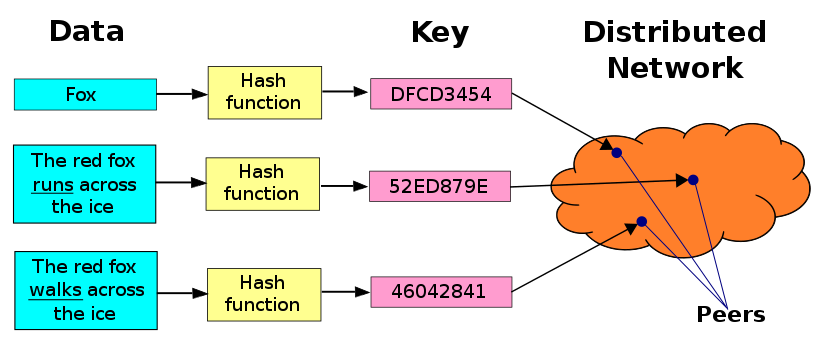
\includegraphics[width=0.6\textwidth]{figures/DHT}
  \caption[Distributed Hash Table] {
    Door het vertalen van data naar een cryptografische sleutel is het mogelijk om aan de hand van de sleutel de data op te vragen aan peers die de data bezitten.
  }
  \label{DHT}
\end{wrapfigure}

\textbf{Consensus}

Consensus is een dynamische manier van het behalen van overeenstemming in een groep. In blockchain implementaties wordt het gebruikt om overeenstemming te behalen over de staat van het netwerk en de volgorde waarin transacties gedaan zijn. Met het consensus algoritme wordt er een zekere mate van veiligheid gewaarborgd, waardoor het voor een kwaadwillende deelnemer (bijna) onmogelijk dient te zijn om het netwerk te beïnvloeden. Het kan voorkomen dat een kwaadwillende deelnemer probeert het netwerk te beïnvloeden waardoor er tegenstrijdige consensus kan optreden en een \gls{fork} ontstaat in het netwerk.

\textbf{Fork}

Een \gls{fork} is een splitsing in het netwerk die veroorzaakt is door een verandering in het protocol of door het toedoen van kwaadwillende deelnemer(s). Er zijn hiervoor twee categorieën \glspl{fork}, een \gls{hard_fork} en een \gls{soft_fork}.

\paragraph{Soft fork}

is een verandering in het netwerk die terugwaartse compatibiliteit heeft met eerdere versies van het protocol. Als voorbeeld kan er voor gekozen worden dat in plaats van blocks een limiet hebben van 1MB, de regel aangepast wordt zodat blocks een grootte van 500K moeten hebben. Als een \gls{soft_fork} verkeerd gaat is het nog steeds mogelijk dat er een \gls{hard_fork} optreed \citep[Soft Fork]{coindesk:forks}.

\paragraph{Hard fork}

is een protocol update waarbij een nieuwe regel geïntroduceerd wordt, waardoor het netwerk geen compatibiliteit heeft met oudere versies. Dit zorgt ervoor dat deelnemers in het netwerk die een oudere versie hebben, de nieuwe transacties als invalide beschouwen. Een voorbeeld van een regel waarbij een \gls{hard_fork} ontstaat is bijvoorbeeld het ophogen van de block grootte naar 2MB in plaats van 1MB \citep[Hard Fork]{coindesk:forks}. 

\newpage
\textbf{\Glspl{node}}

Alhoewel de structuur van een Blockchain dezelfde structuur afdwingt voor de \glspl{node} in het netwerk, kunnen zij een verschillende rol spelen. Alle \glspl{node} binnen het netwerk valideren, verspreiden en ontdekken en onderhouden connecties met andere \glspl{node} binnen het netwerk. In fig. \ref{blockchain_node_types} is te zien welke services een  \gls{full_node} in het Bitcoin netwerk aanbiedt. 

\begin{wrapfigure}{r}{0.4\textwidth}
  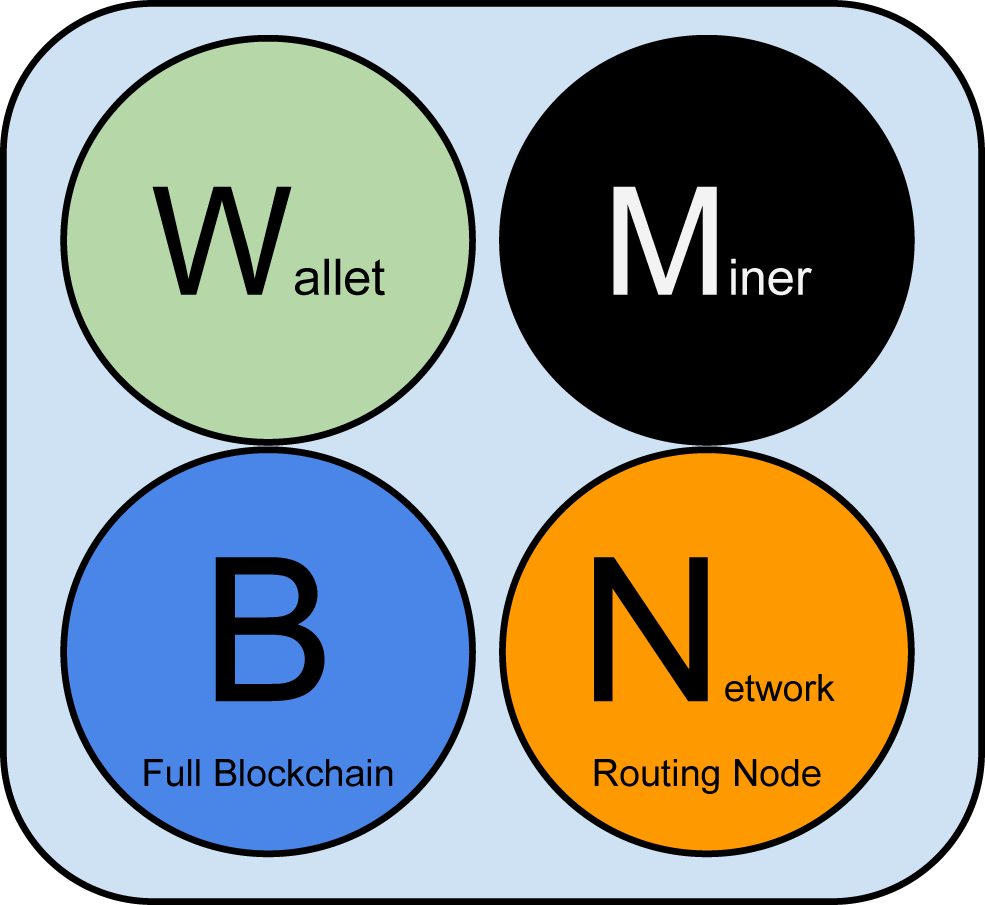
\includegraphics[width=0.4\textwidth]{figures/bitcoin_node_types}
  \caption[Bitcoin Node functionaliteiten] {
    Een bitcoin netwerk node die alle functies bevat: wallet, mining, blockchain database en netwerk routing, \citep[p.~172]{Antonopoulos:2014:MBU:2695500}.
  }
  \label{blockchain_node_types}
\end{wrapfigure}

Een \textbf{\gls{full_node}} is een collectie van functies, namelijk routing, de blockchain database, het mining proces en wallet services en bevat een gehele kopie van de actuele blockchain. Een \textbf{\gls{wallet_node}} is een deelnemer in het netwerk die een subset van de gehele blockchain bevat om transacties te versturen, verifiëren en ontvangen. De \textbf{\glspl{mining_node}} concurreren voor het creëren van een nieuw block door het uitvoeren van het Proof-of-Work algoritme. 

Alle \glspl{node} binnen het netwerk bieden gelijke diensten aan en kunnen gebruik maken van dezelfde diensten terwijl ze samenwerken door middel van een consensus protocol.

De verschillende services binnen het netwerk en de \gls{node} types die hieraan meewerken is dan ook een architecturale keuze over de indeling van het \acrshort{P2P} netwerk.
